\documentclass[11pt,aspectratio=169]{beamer}
\usetheme{Boadilla}
\usecolortheme{seahorse}
\setbeamertemplate{navigation symbols}{}
\setbeamertemplate{footline}[frame number]
\usepackage{graphicx,booktabs,amsmath}
\graphicspath{{../../../fullsim_analysis/results/bench/2026-10-27/}}
\newcommand{\results}{../../../fullsim_analysis/results/bench/2026-10-27}

\title{The Citiroc front end on the bench}
\subtitle{Pedestal noise, hold-delay scan and single-photoelectron calibration: session of 27 October 2026}
\author{J.\,J.~Gómez-Cadenas}
\date{28 October 2026}

\begin{document}

\begin{frame}
\titlepage
\end{frame}

\begin{frame}{The session of 27 October 2026}
\begin{itemize}
\item Three A5202 boards, 1, 2 and 4, each with two Citiroc~1A and a 64-channel SiPM matrix,
  connected through the CAEN adapter boards and running the upgraded FPGA firmware
  (0xa7070800). The DAQ reads them on one chain as boards 0, 1, 2.
\item The three menus of the calibration programme:
  \begin{enumerate}
  \item \textbf{Pedestal noise}, SiPMs below breakdown: runs 91--99, three boards.
  \item \textbf{Hold-delay scan}, SiPMs at 5~V of overvoltage: staircase 100 and hold-delay
    scans 101--106, board 1.
  \item \textbf{Single-photoelectron calibration} with the periodic trigger: runs 108--112
    at 5, 4 and 3~V of overvoltage, three boards; staircases 113--115, board 1.
  \end{enumerate}
\item Every run with its settings, temperatures and incidents in the logbook of the day.
\end{itemize}
\end{frame}

\section{Menu 1: pedestal noise}

\begin{frame}{Menu 1: data}
\centering
\begin{tabular}{llll}
\toprule
Runs & Purpose & HG shaping & HoldDelay \\
\midrule
91--93 & shaping & 25, 50, 87.5 ns & 0 \\
94--98 & window & 25 ns & 96--496 ns \\
99 & stability & 25 ns & 0 \\
\bottomrule
\end{tabular}

\bigskip
\raggedright
SiPMs at 36.5~V, below breakdown; periodic trigger at 1~kHz; 10\,000 events per board and run;
preamplifier gains 55; peak-stretch mode; low gain at 87.5~ns. Boards 1, 2 and 4, read by the
DAQ as 0, 1, 2.
\end{frame}

\begin{frame}{Menu 1: method}
Channel $i$, event $e$, high-gain value $v_i(e)$:
\begin{align*}
p_i &= \operatorname{median}_e v_i(e), \quad d_i(e) = v_i(e) - p_i, \quad
\mathrm{CM}(e) = \tfrac{1}{n}\textstyle\sum_i d_i(e),\\
d_i(e) &= b_i\,\mathrm{CM}(e) + r_i(e),\\
\sigma_\mathrm{tot}^2 &= \langle d_i^2\rangle = \sigma_\mathrm{coh}^2 + \sigma_\mathrm{inc}^2,
\quad \sigma_\mathrm{coh}^2 = \langle b_i^2\,\mathrm{CM}^2\rangle, \quad
\sigma_\mathrm{inc}^2 = \langle r_i^2\rangle.
\end{align*}
\begin{itemize}
\item $p_i$ pedestal, $d_i$ deviation, $\mathrm{CM}$ common mode of the $n$ channels of the
  chip read at the same trigger, $b_i$ slope of the channel against it, $r_i$ incoherent part;
  $\langle\,\rangle$ over channels and events.
\item Jumps of the chip ($|\mathrm{CM}| > 6\,s_\mathrm{CM}$) and outliers
  ($|d_i - \mathrm{CM}| > 5\,s_i$) set aside; $s$ the robust width, 1.4826 times the median
  absolute deviation.
\item A \emph{blind channel} takes no common mode ($b_i < 0.75$) and is excluded from $n$.
\end{itemize}
\end{frame}

\begin{frame}{Noise of every channel}
\begin{columns}
\column{0.6\textwidth}
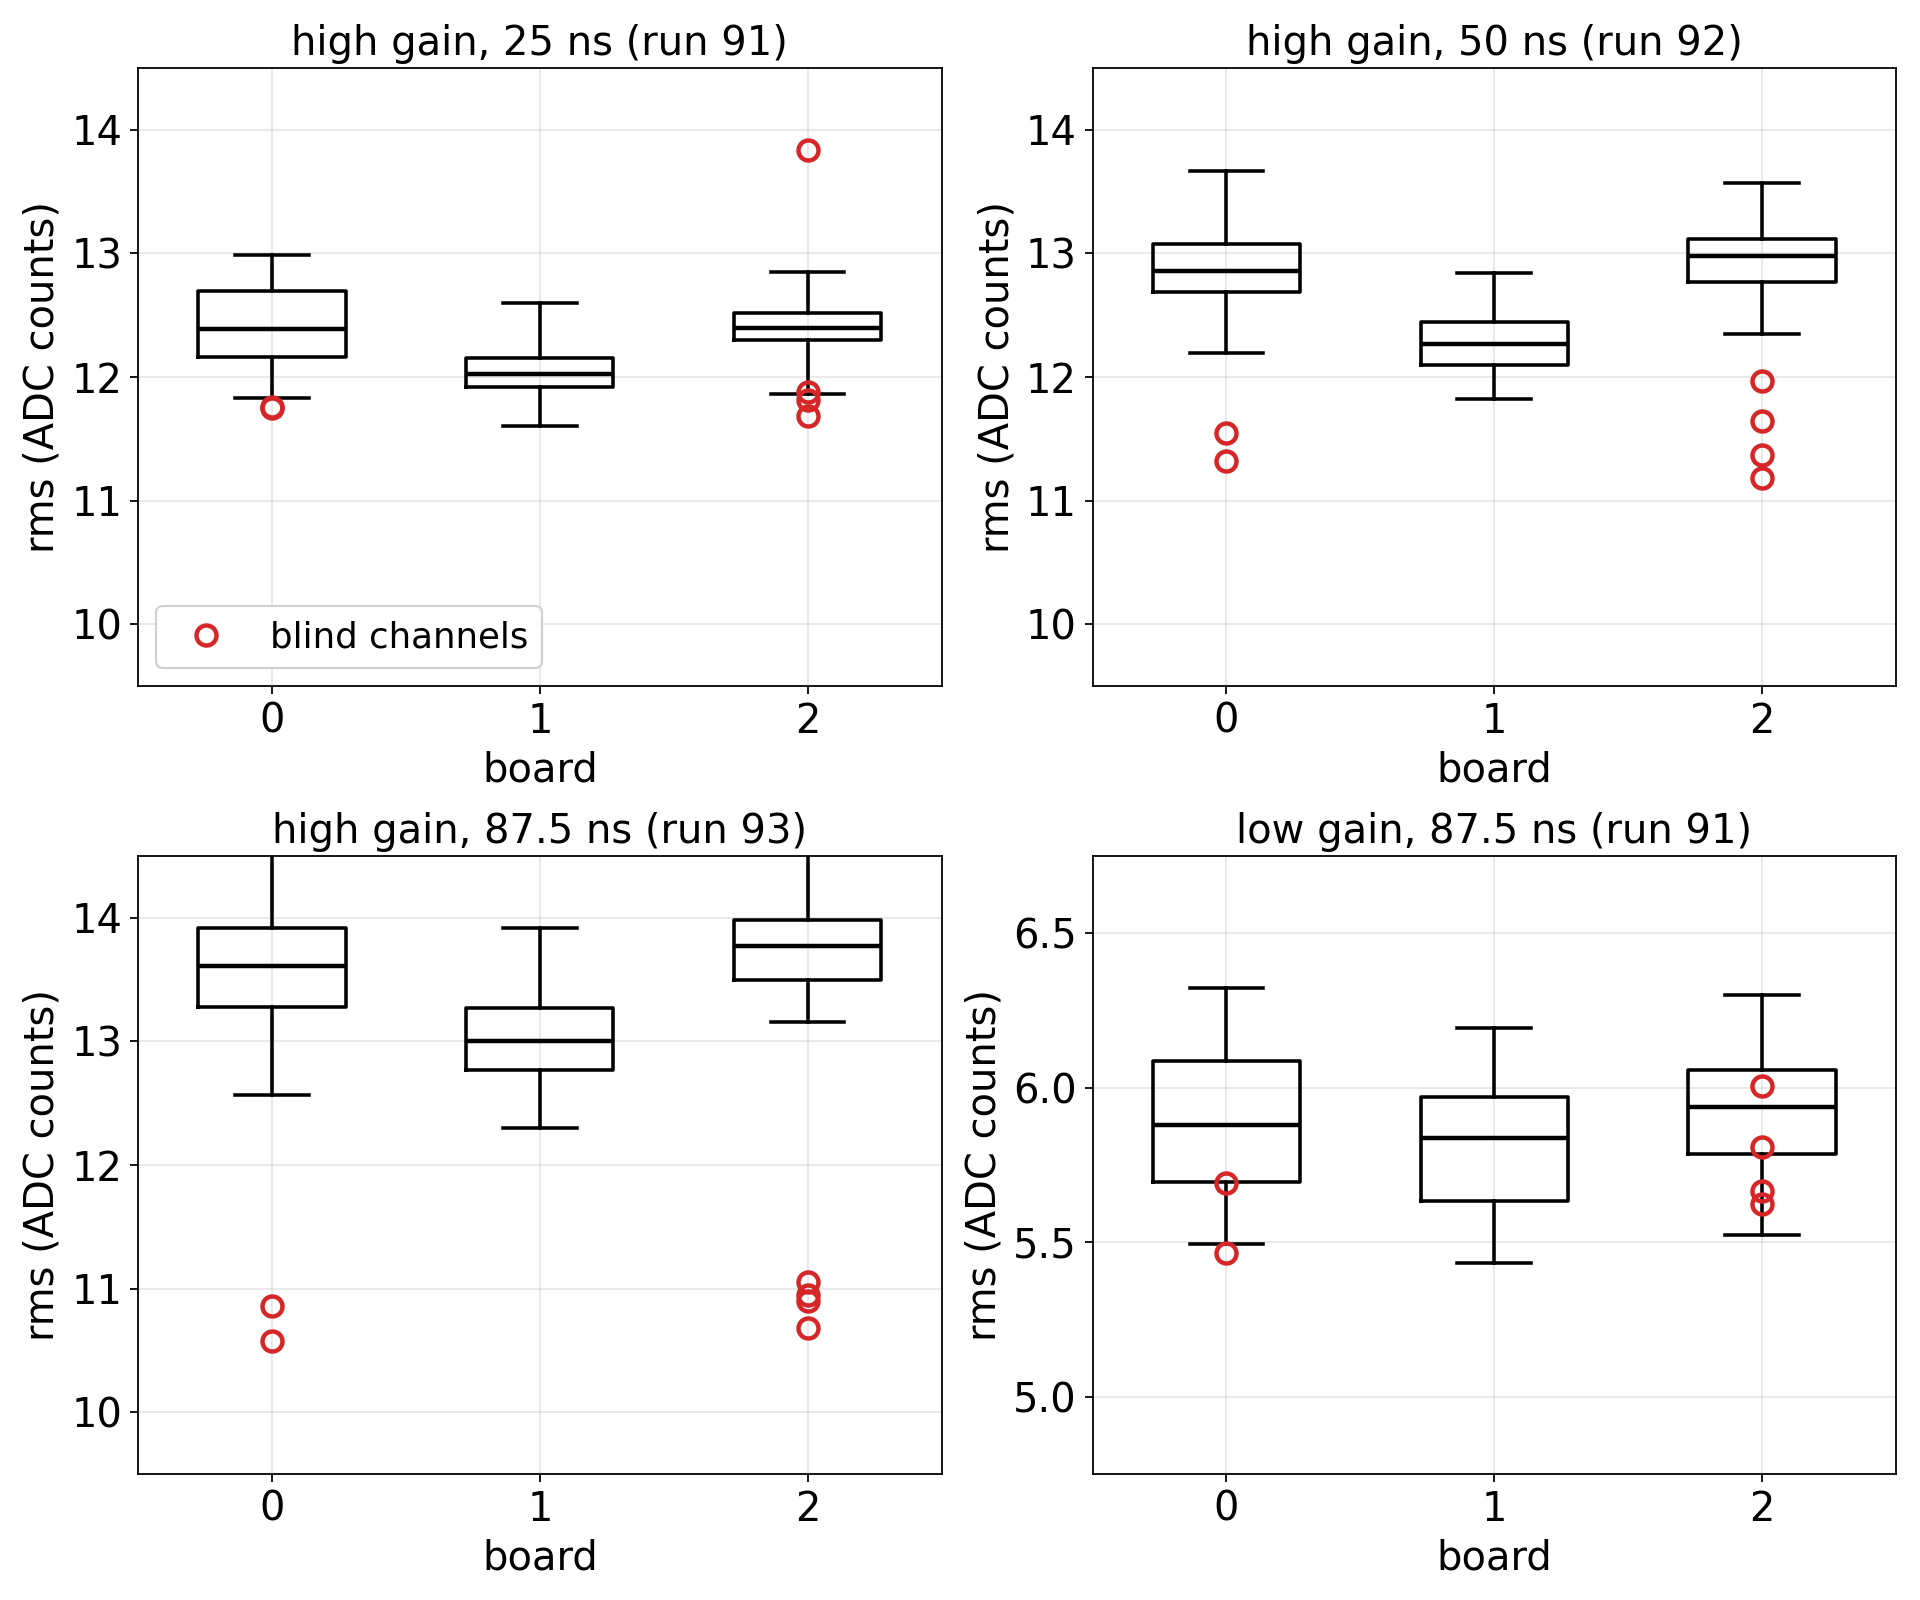
\includegraphics[width=\textwidth]{bench_rms.png}
\column{0.4\textwidth}
\begin{itemize}
\item Every channel of the three boards is read; $100 < p_i < 300$.
\item Rms at 25~ns: 12.0--12.4 counts in the median of each board (high gain), spread of
  about 1~count over the 64 channels; 5.9 in the low gain.
\item Red: the blind channels.
\end{itemize}
\end{columns}
\end{frame}

\begin{frame}{Coherent and incoherent noise per chip}
\begin{columns}
\column{0.55\textwidth}
\centering
\scriptsize
\input{\results/menu1_chips.tex}

\medskip
Run 91: high gain, 25~ns, HoldDelay 0, ADC counts; low gain at 87.5~ns.
\column{0.45\textwidth}
\begin{itemize}
\item Six chips: $11.9 \le \sigma_\mathrm{tot} \le 12.7$, $5.9 \le \sigma_\mathrm{coh} \le 6.7$,
  $10.3 \le \sigma_\mathrm{inc} \le 10.8$.
\item The coherent part carries 24--28\% of the variance.
\item Correlation of the common modes: 0.59--0.64 between the two chips of a board, zero
  between boards.
\item No jump of any chip in the nine runs.
\end{itemize}
\end{columns}
\end{frame}

\begin{frame}{Dependence on the shaping time}
\begin{columns}
\column{0.6\textwidth}
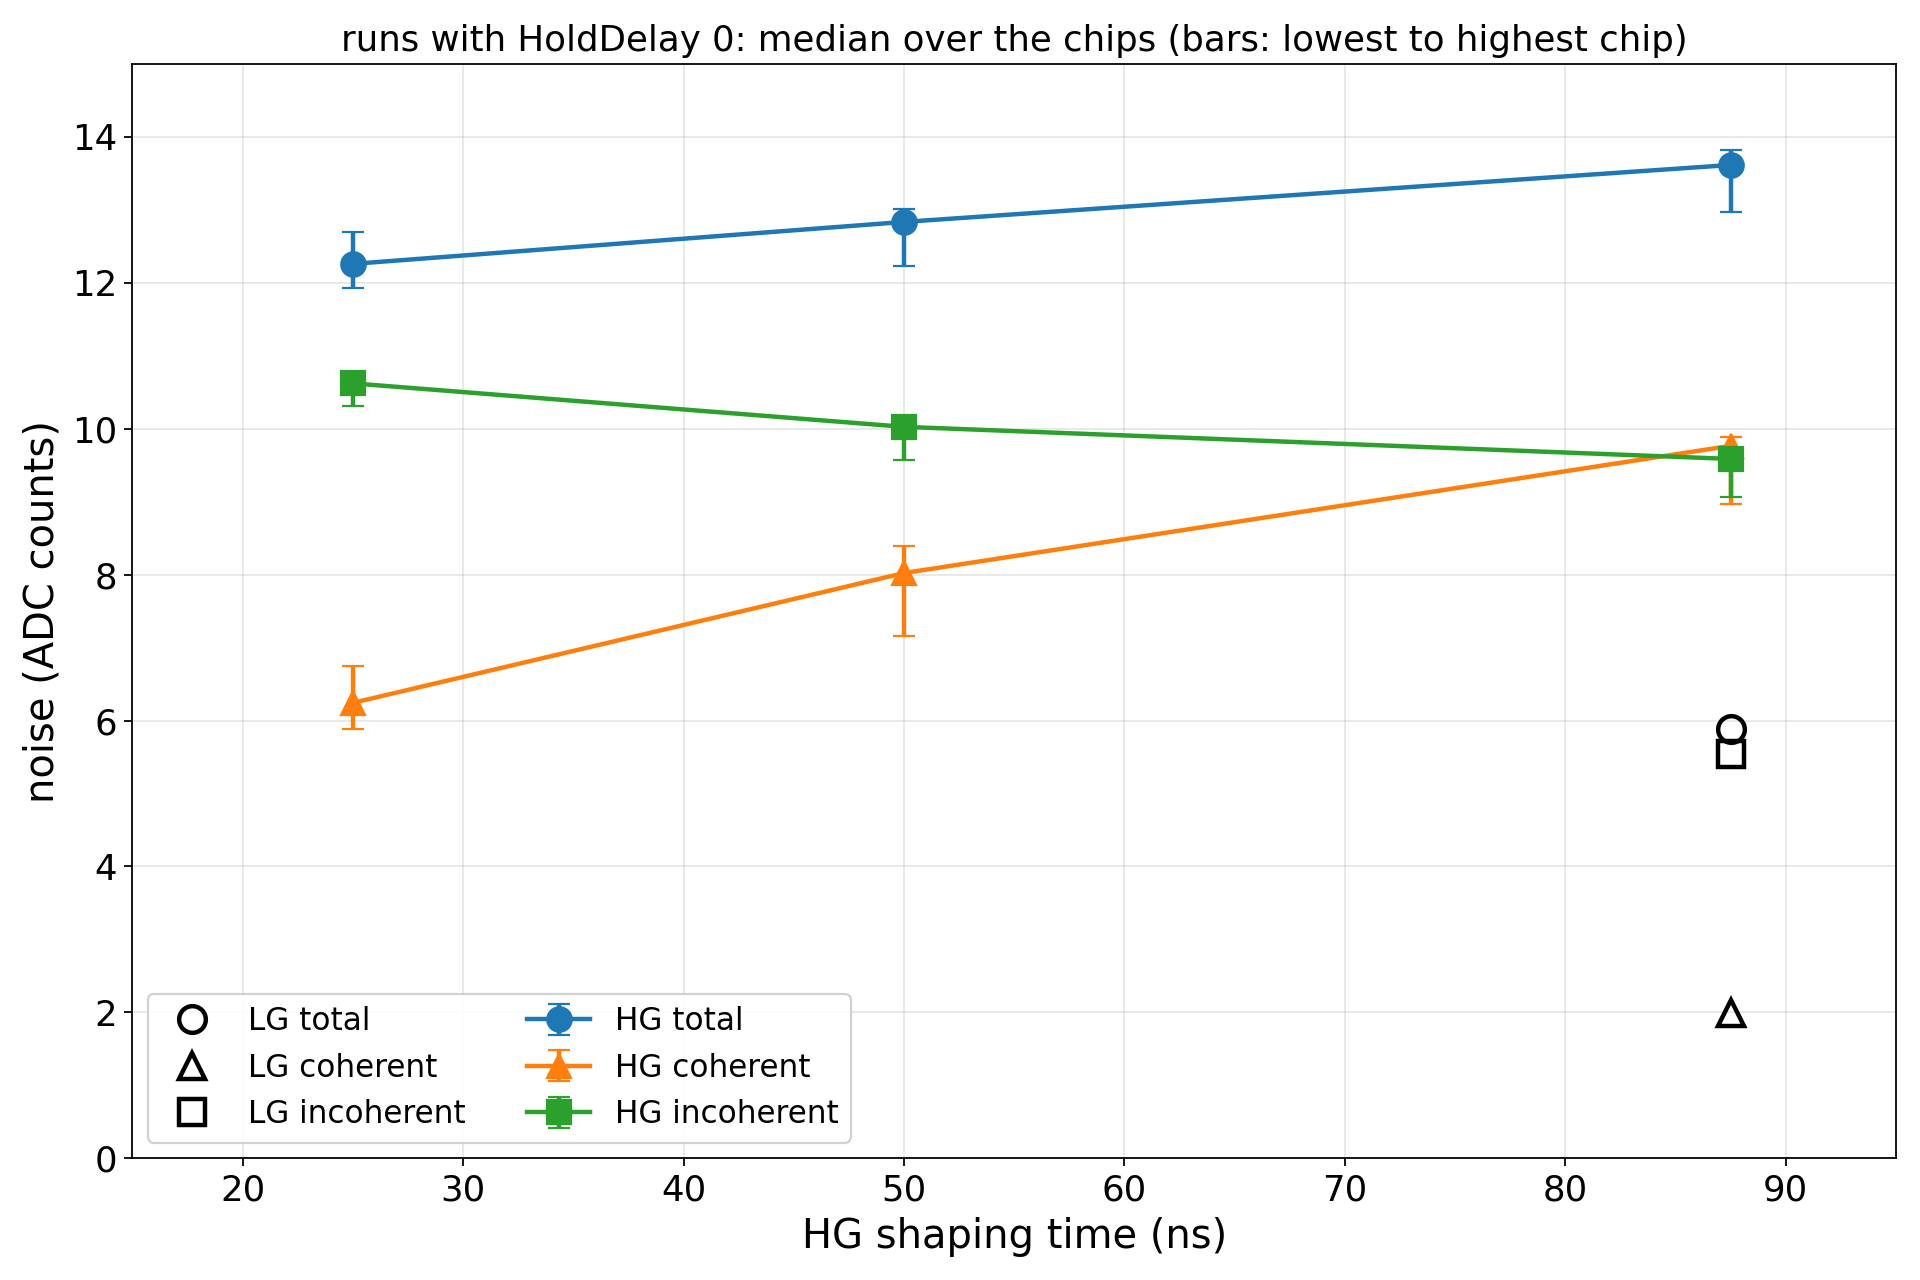
\includegraphics[width=\textwidth]{noise_vs_shaping_data.png}
\column{0.4\textwidth}
\begin{itemize}
\item Total 12.3, 12.8, 13.6 counts at 25, 50, 87.5~ns (median over the chips).
\item $\sigma_\mathrm{coh}$ grows from 6.2 to 9.8 between 25 and 87.5~ns; $\sigma_\mathrm{inc}$
  falls from 10.6 to 9.6.
\item Low gain: 0.48, 0.46, 0.43 of $\sigma_\mathrm{tot}$ of the high gain.
\end{itemize}
\end{columns}
\end{frame}

\begin{frame}{Dependence on the hold delay}
\begin{columns}
\column{0.5\textwidth}
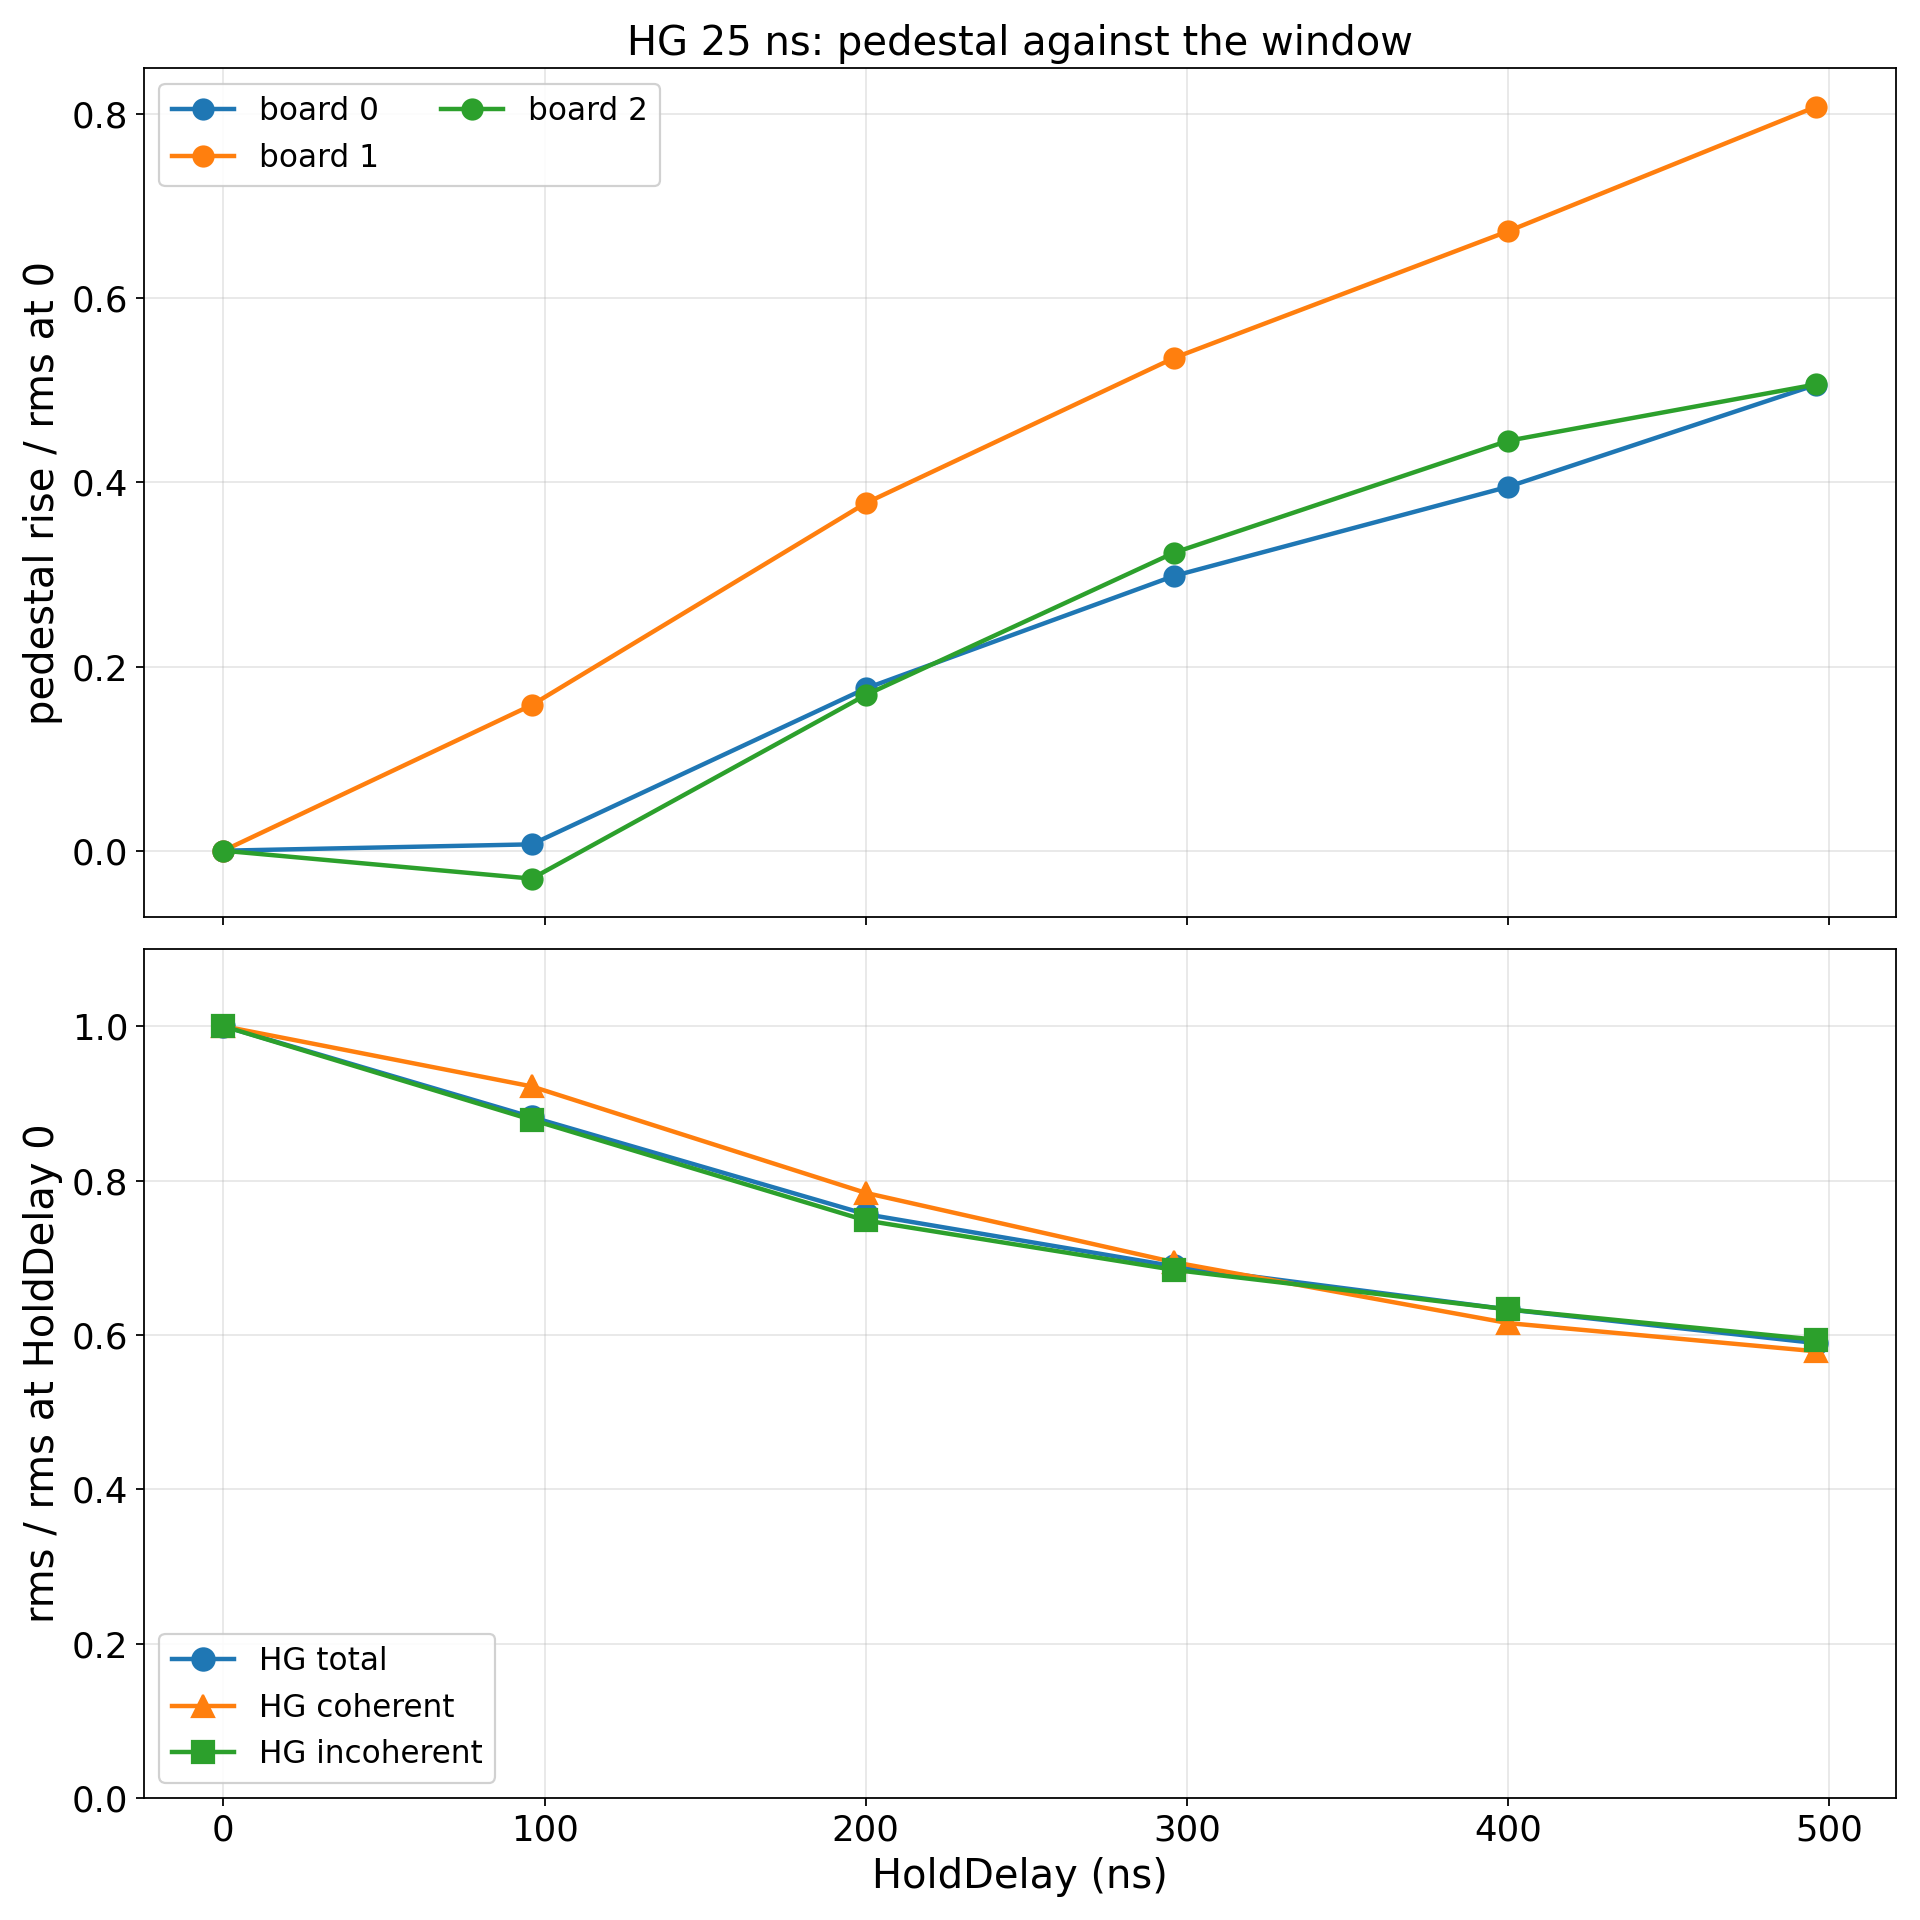
\includegraphics[width=\textwidth]{noise_vs_holddelay_data.png}
\column{0.5\textwidth}
\begin{itemize}
\item Peak-stretch mode: the stored value is the maximum of the shaped signal over the window.
\item Both components narrow together: 1.00, 0.88, 0.76, 0.69, 0.63, 0.59 at 0, 96, 200, 296,
  400, 496~ns.
\item The pedestal rises with the window: 0.62 of $\sigma_\mathrm{tot}(0)$ at 496~ns in the
  median; 0.81 on board 2, 0.51 on boards 1 and 4, where the rise starts after 96~ns.
\end{itemize}
\end{columns}
\end{frame}

\begin{frame}{Blind channels}
\begin{columns}
\column{0.6\textwidth}
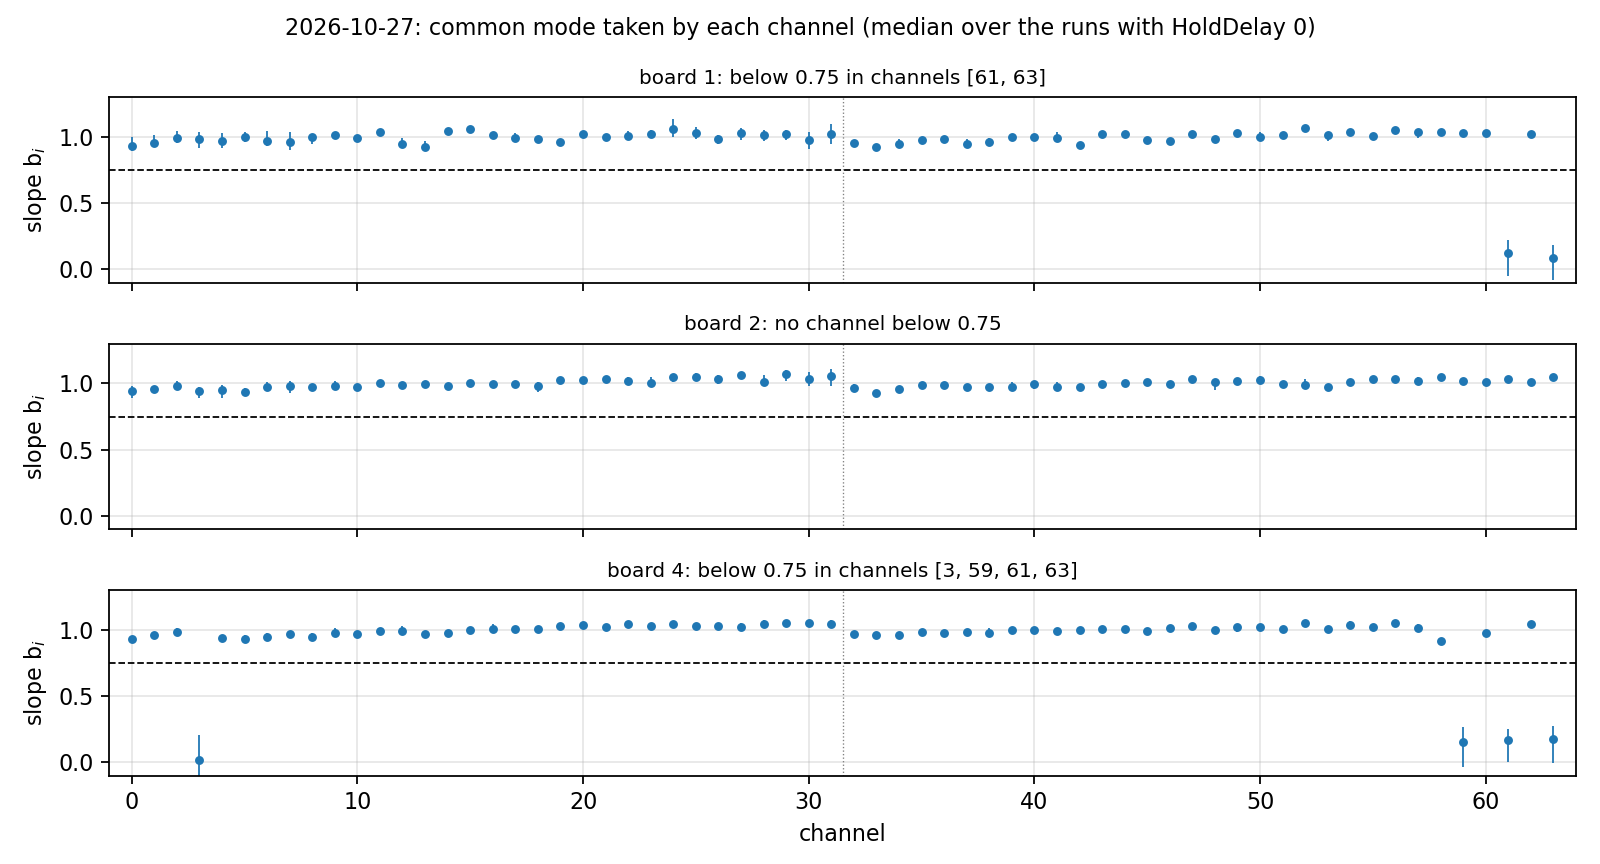
\includegraphics[width=\textwidth]{bench_slopes.png}
\column{0.4\textwidth}
\begin{itemize}
\item The common mode enters the chip through the SiPMs: a channel whose SiPM signal does not
  reach the chip takes a slope $b_i$ well below one.
\item Board 1: channels 61 and 63 ($b_i < 0.2$). Channel 62, blind on 23 October, takes the
  full common mode.
\item Board 4: channels 3, 59, 61 and 63.
\item Board 2: none. Every other channel: $b_i > 0.85$.
\end{itemize}
\end{columns}
\end{frame}

\begin{frame}{Values frozen for the noise model}
High gain, preamplifier gain 55, ADC counts:
\medskip

\centering
\small
\begin{tabular}{lp{0.5\textwidth}}
\toprule
per channel, 25 ns, HoldDelay 0 & $\sigma_\mathrm{tot} = 12.3$, $\sigma_\mathrm{coh} = 6.2$, $\sigma_\mathrm{inc} = 10.6$ \\
against the shaping (25, 50, 87.5 ns) & $\sigma_\mathrm{coh} = 6.2, 8.0, 9.8$; $\sigma_\mathrm{inc} = 10.6, 10.0, 9.6$ \\
against the hold delay (0--496 ns, 25 ns) & both components scaled by 1.00, 0.88, 0.76, 0.69, 0.63, 0.59 \\
coherent component & common to the 64 channels of a board; correlation 0.6 between its chips, 0 between boards \\
low gain, 87.5 ns & 0.46 of $\sigma_\mathrm{tot}$ of the high gain \\
blind channels & board 1: 61, 63; board 4: 3, 59, 61, 63 \\
\bottomrule
\end{tabular}
\medskip

\raggedright
The sessions of 22 and 23 October (five boards, both adapter boards, both firmwares) gave the
same values. The conversion to photoelectrons takes the single-photoelectron gain from menu 3.
\end{frame}

\section{Menu 2: threshold and hold delay}

\begin{frame}{Menu 2: data}
\begin{itemize}
\item Board 1, SiPMs at 43~V (5~V of overvoltage), threshold 185, preamplifier gains 55,
  peak-stretch mode.
\item \textbf{Staircase} (scan 100): trigger rate of the 64 channels against the threshold of
  the discriminator, 150--300 DAC units, 0.5~s per point, 25~ns.
\item \textbf{Hold-delay scans}: the trigger limited to one channel (the shooting channel), the
  high-gain spectrum of every channel stored at each delay, 10\,000 events per delay.
\end{itemize}
\medskip
\centering
\small
\begin{tabular}{llll}
\toprule
Scan & Shooting channel & HG shaping & HoldDelay \\
\midrule
101 & 0 & 25 ns & 0--248 ns, steps of 8 \\
102, 103 & 0 & 50 ns & 0--496 ns, steps of 16 \\
104, 105, 106 & 20, 40, 60 & 25 ns & 0--248 ns, steps of 8 \\
\bottomrule
\end{tabular}
\medskip

\normalsize
The DAQ applies a new delay with a lag of up to five points: the first points of a scan keep the
values of the previous scan and are left out.
\end{frame}

\begin{frame}{Threshold: the staircase at 5 V}
\begin{columns}
\column{0.6\textwidth}
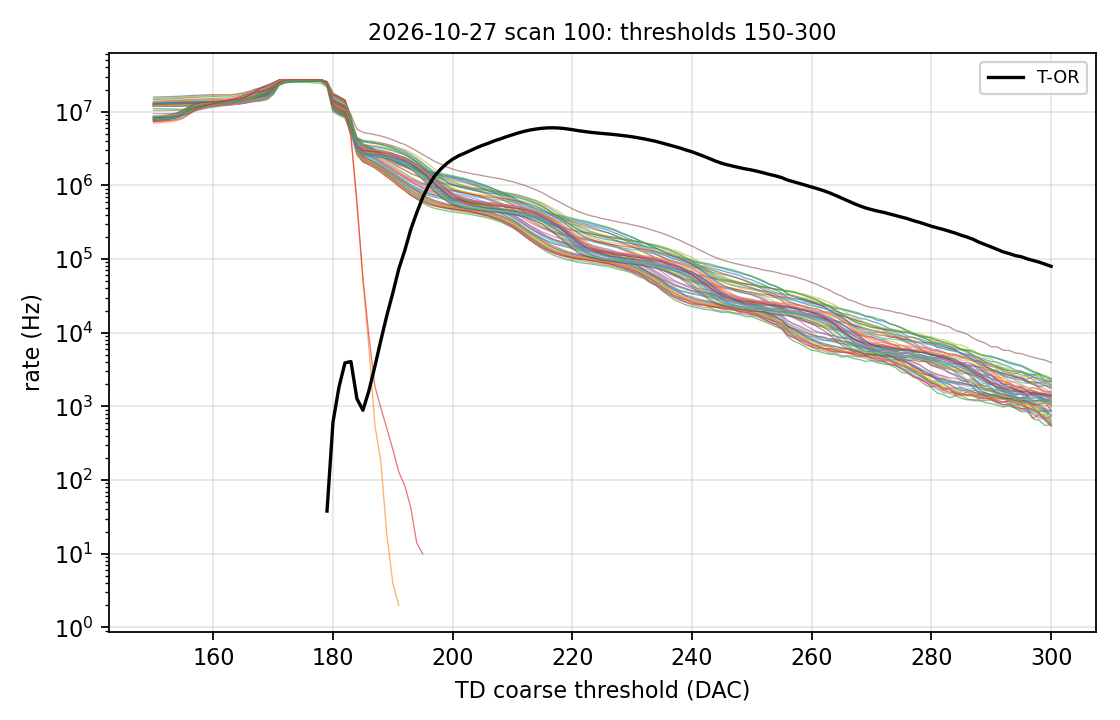
\includegraphics[width=\textwidth]{staircase_100.png}
\column{0.4\textwidth}
\begin{itemize}
\item Edge of the noise of the fast shaper at 179--182 DAC units.
\item Above it the rate falls in steps of one photoelectron: 20 units per photoelectron.
\item 30 units above the edge: dark pulses at $4.4\times 10^{5}$~Hz (median).
\item Channels 61 and 63 fall to a few hertz within 10 units: no SiPM signal.
\item The threshold of 185 is below one photoelectron.
\end{itemize}
\end{columns}
\end{frame}

\begin{frame}{Response of the peak detector}
\begin{columns}
\column{0.62\textwidth}
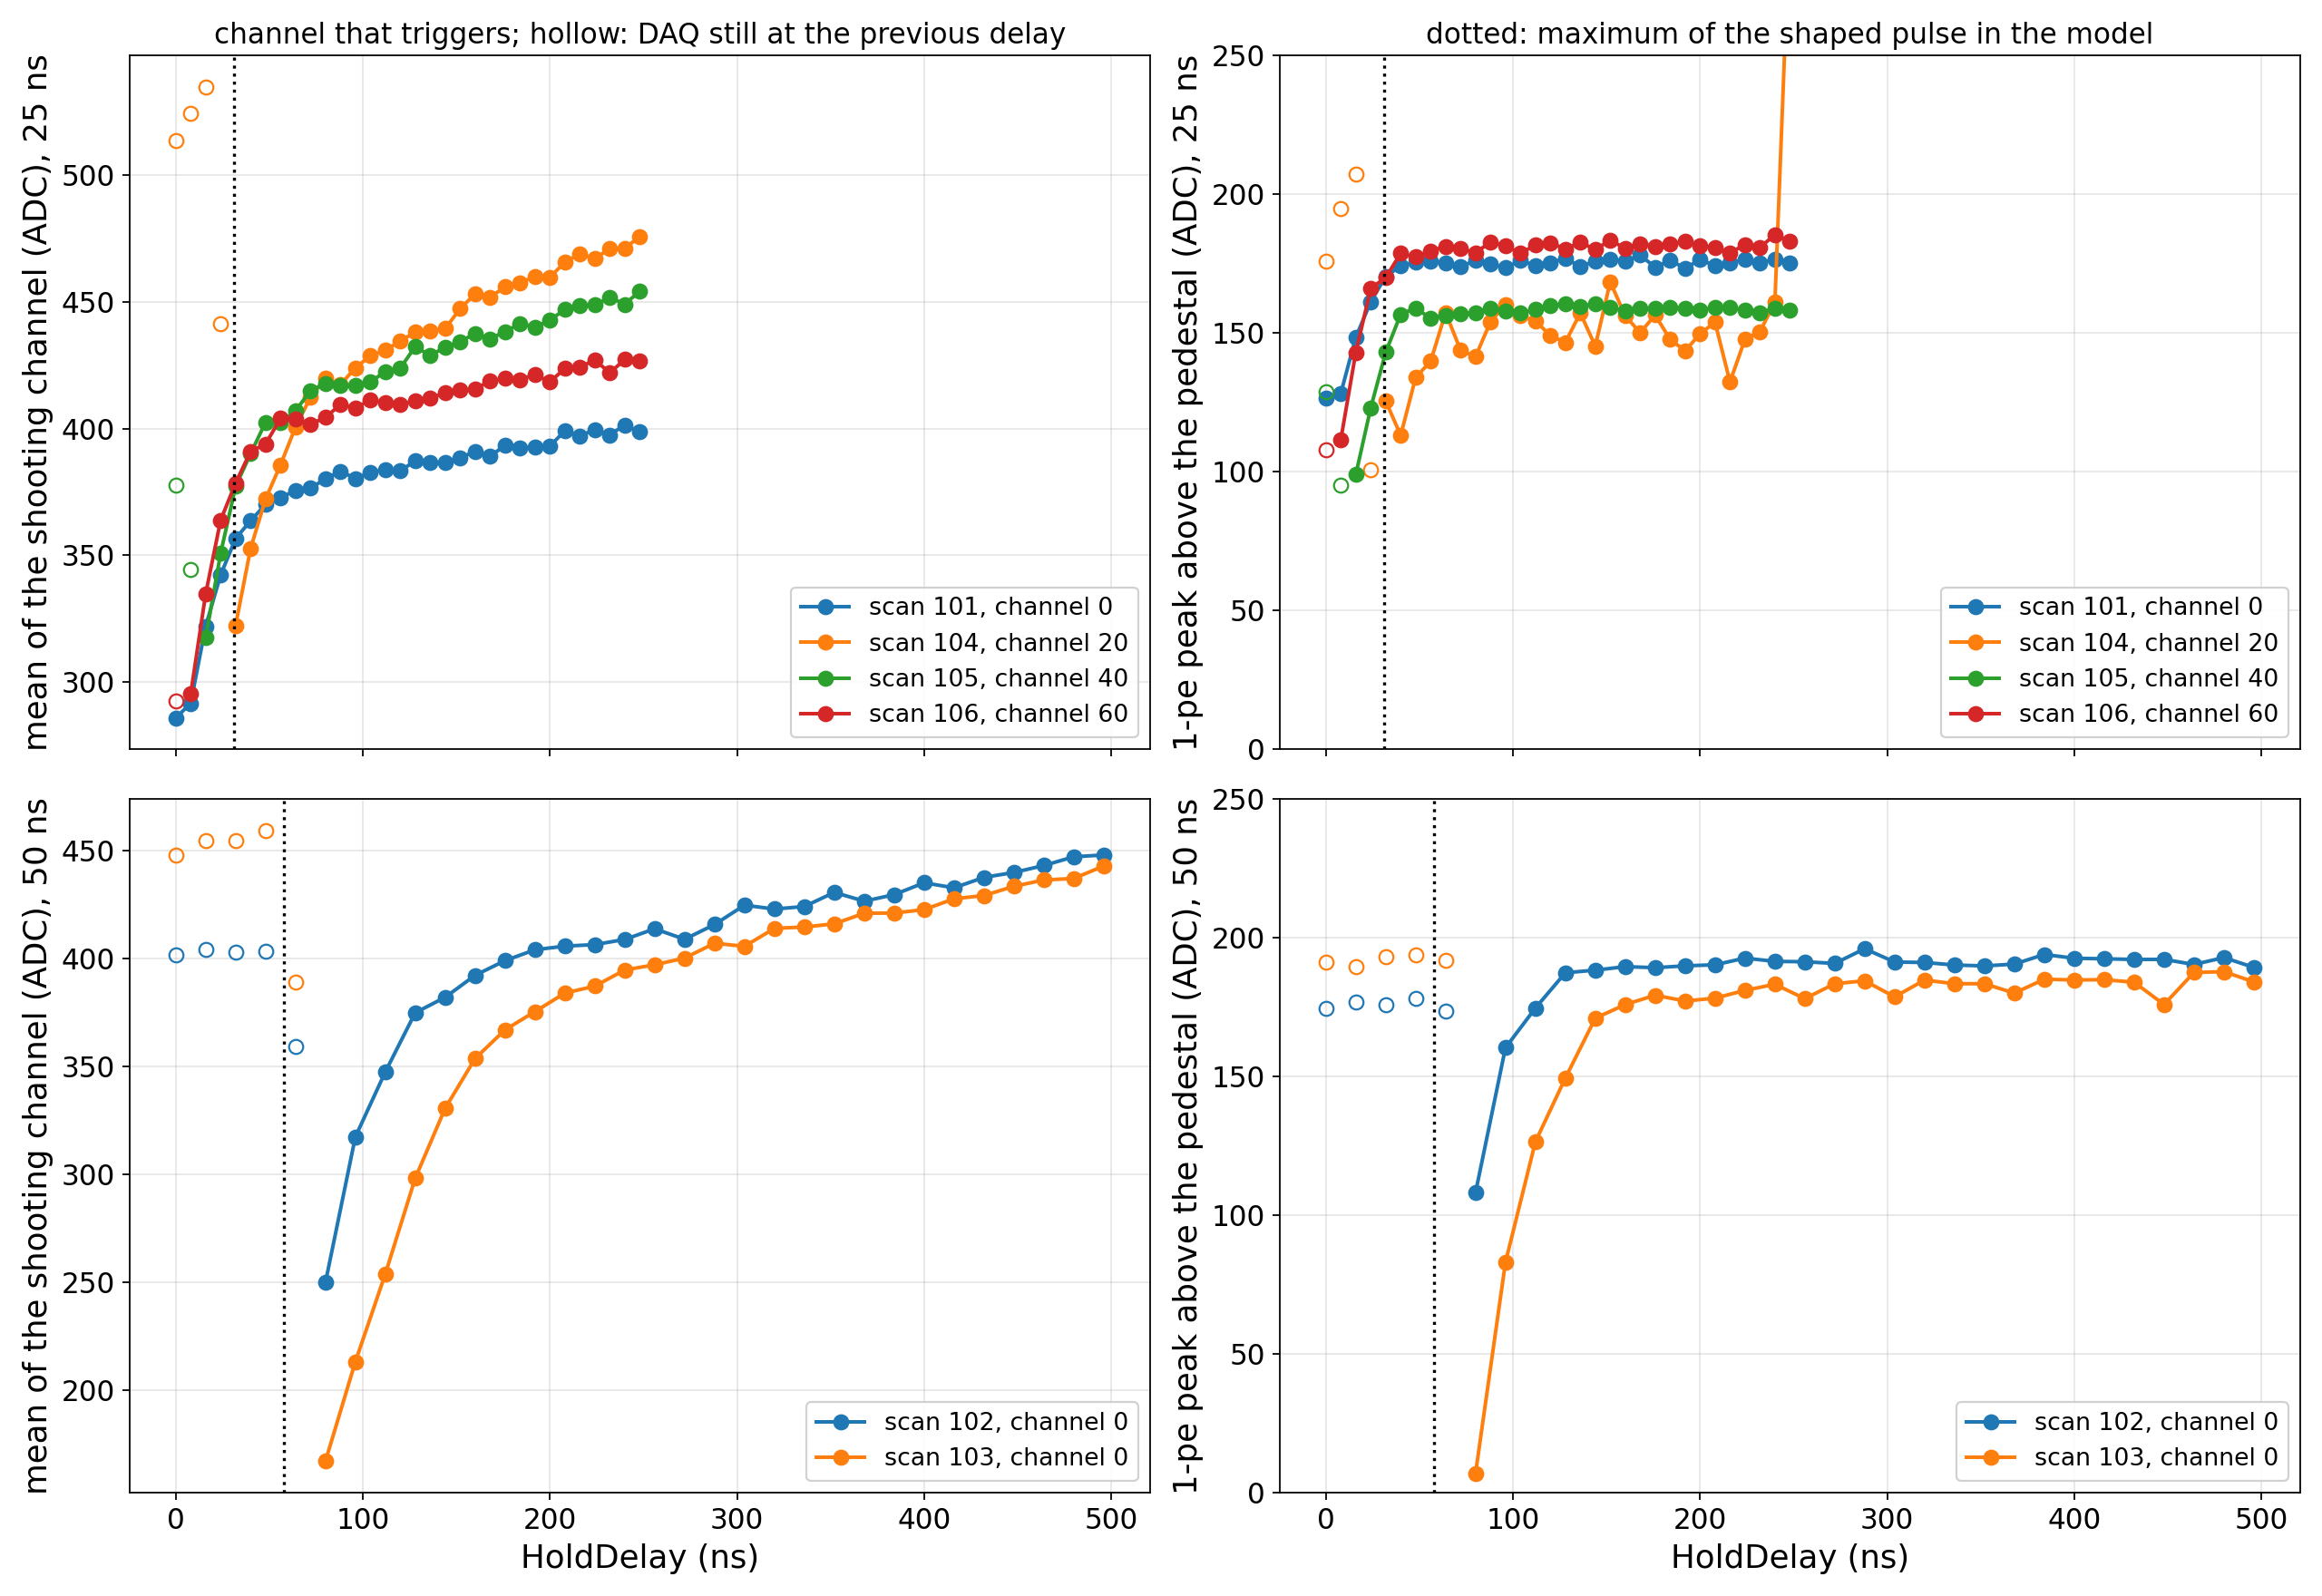
\includegraphics[width=\textwidth]{hold_scan_response.png}
\column{0.38\textwidth}
\begin{itemize}
\item Right: the 1-pe peak of the shooting channel, the response to a single avalanche. Left:
  its mean, which keeps growing with the dark pulses in the window.
\item 25~ns: plateau from 32--40~ns, flat to 248~ns; the model puts the maximum of the shaped
  pulse at 31~ns.
\item 50~ns: plateau from 130--160~ns; the model's maximum at 58~ns.
\item Hollow: DAQ still at the previous delay.
\end{itemize}
\end{columns}
\end{frame}

\begin{frame}{Spectra of the shooting channel}
\begin{columns}
\column{0.62\textwidth}
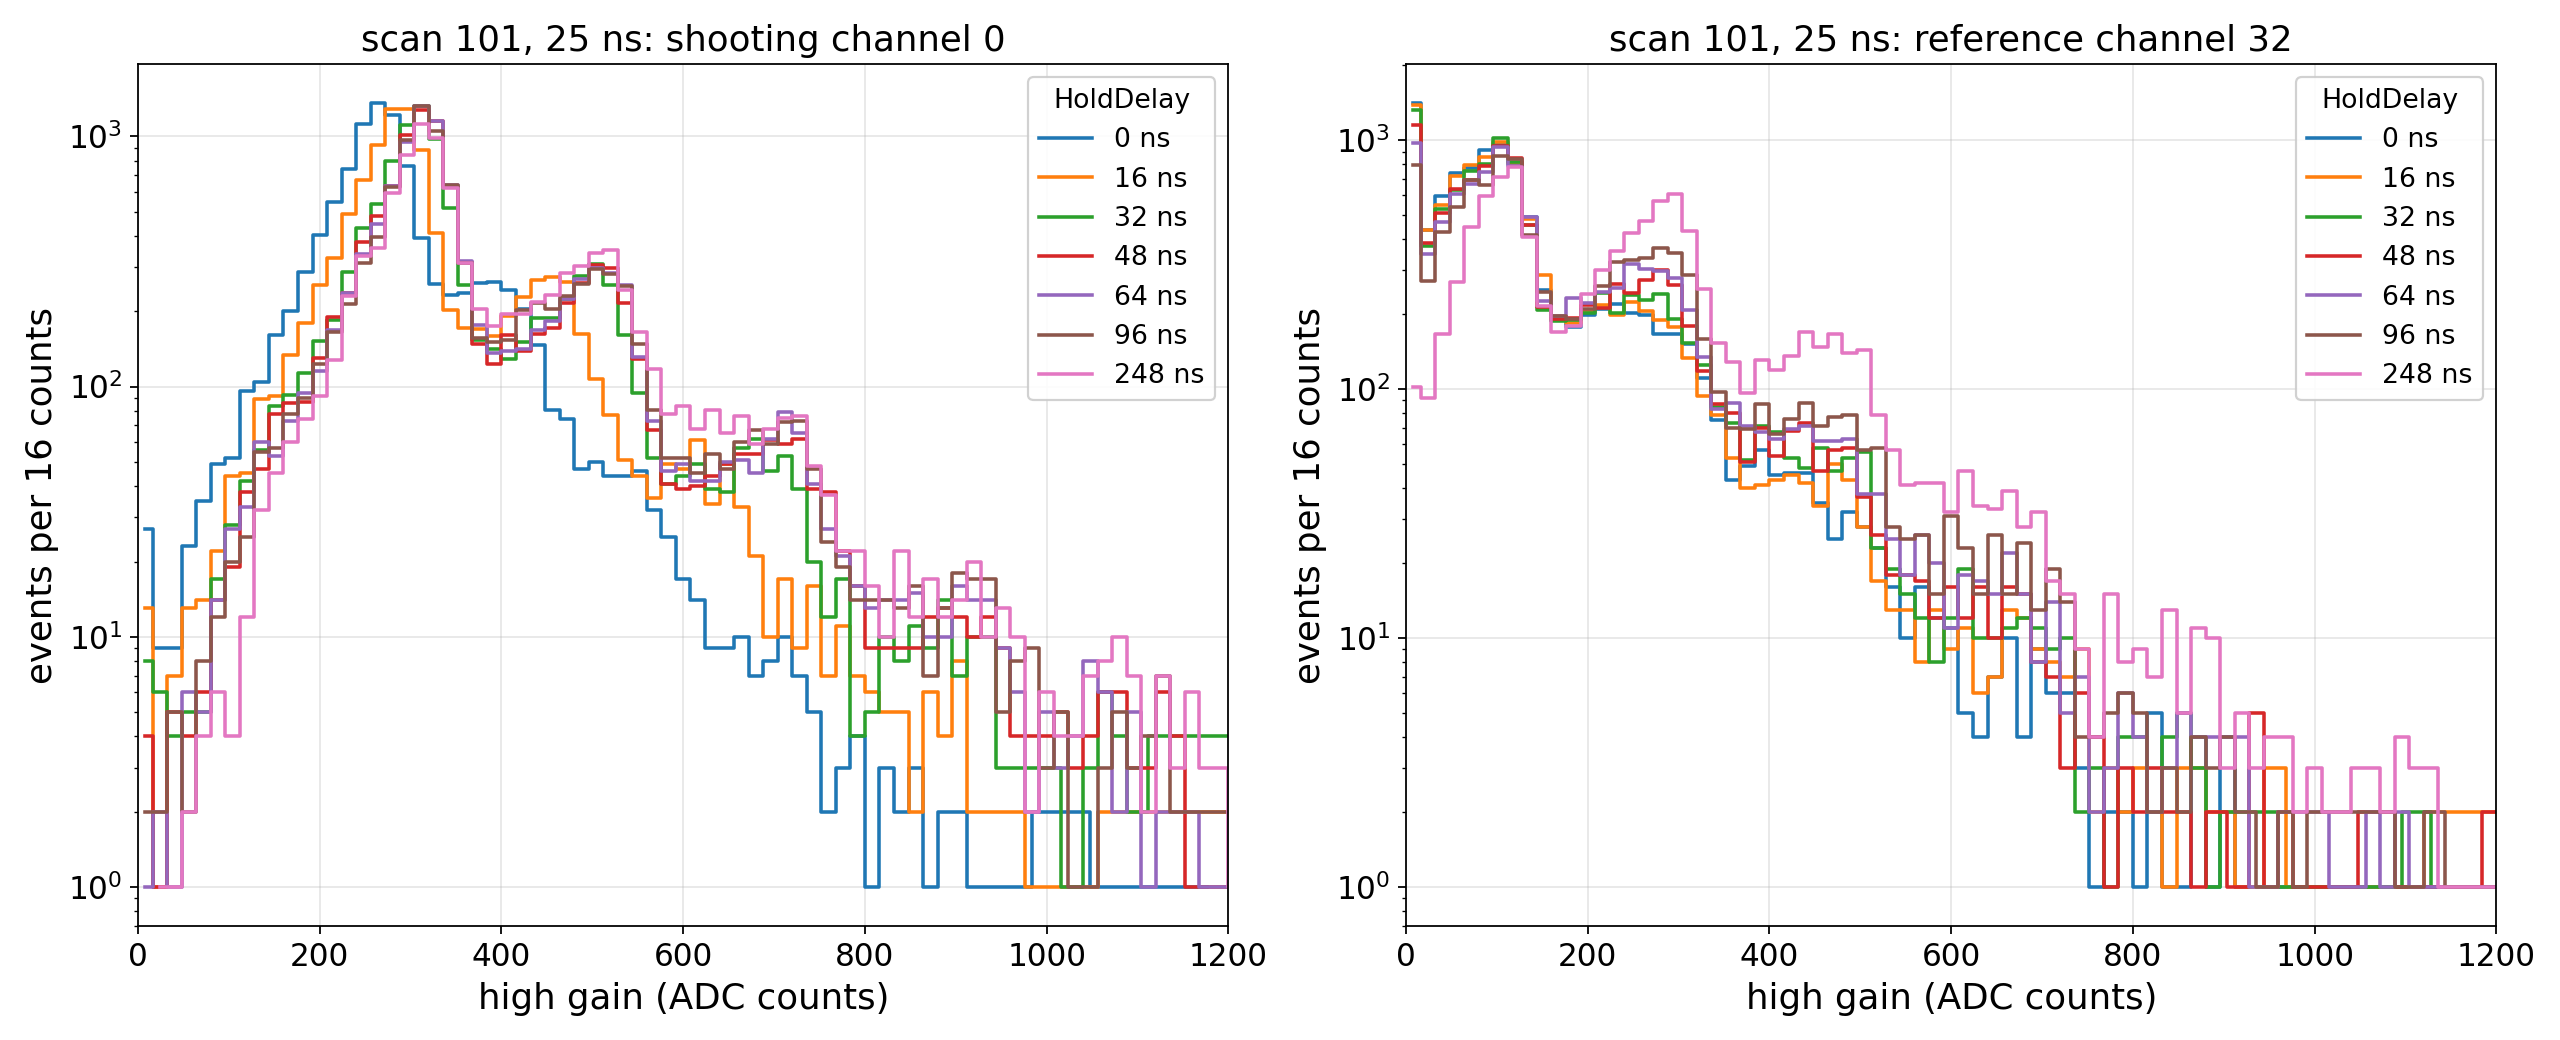
\includegraphics[width=\textwidth]{hold_scan_spectra.png}
\column{0.38\textwidth}
\begin{itemize}
\item Shooting channel 0 at 25~ns: 1-pe peak at 265 counts at delay 0, at 315 from 32~ns on;
  2 and 3~pe at 505 and 700, 190~counts apart.
\item Channel 32, which does not trigger: the pedestal and a ladder of 1, 2, 3~pe that fills as
  the window lengthens.
\end{itemize}
\end{columns}
\end{frame}

\begin{frame}{Knee and gain at 5 V}
\centering
\input{\results/hold_scan_knees.tex}

\medskip
\begin{itemize}
\item Knee: first delay at which the 1-pe peak reaches 95\% of its plateau. Pedestal: below
  breakdown at the same shaping. ADC counts of the high gain.
\item Minimum hold delay: 40~ns at 25~ns of shaping, 160~ns at 50~ns.
\item Gain at 5~V: 150--182 counts per photoelectron at 25~ns in the four channels scanned,
  185--192 at 50~ns.
\end{itemize}
\end{frame}

\begin{frame}{A window at a random time}
\begin{columns}
\column{0.6\textwidth}
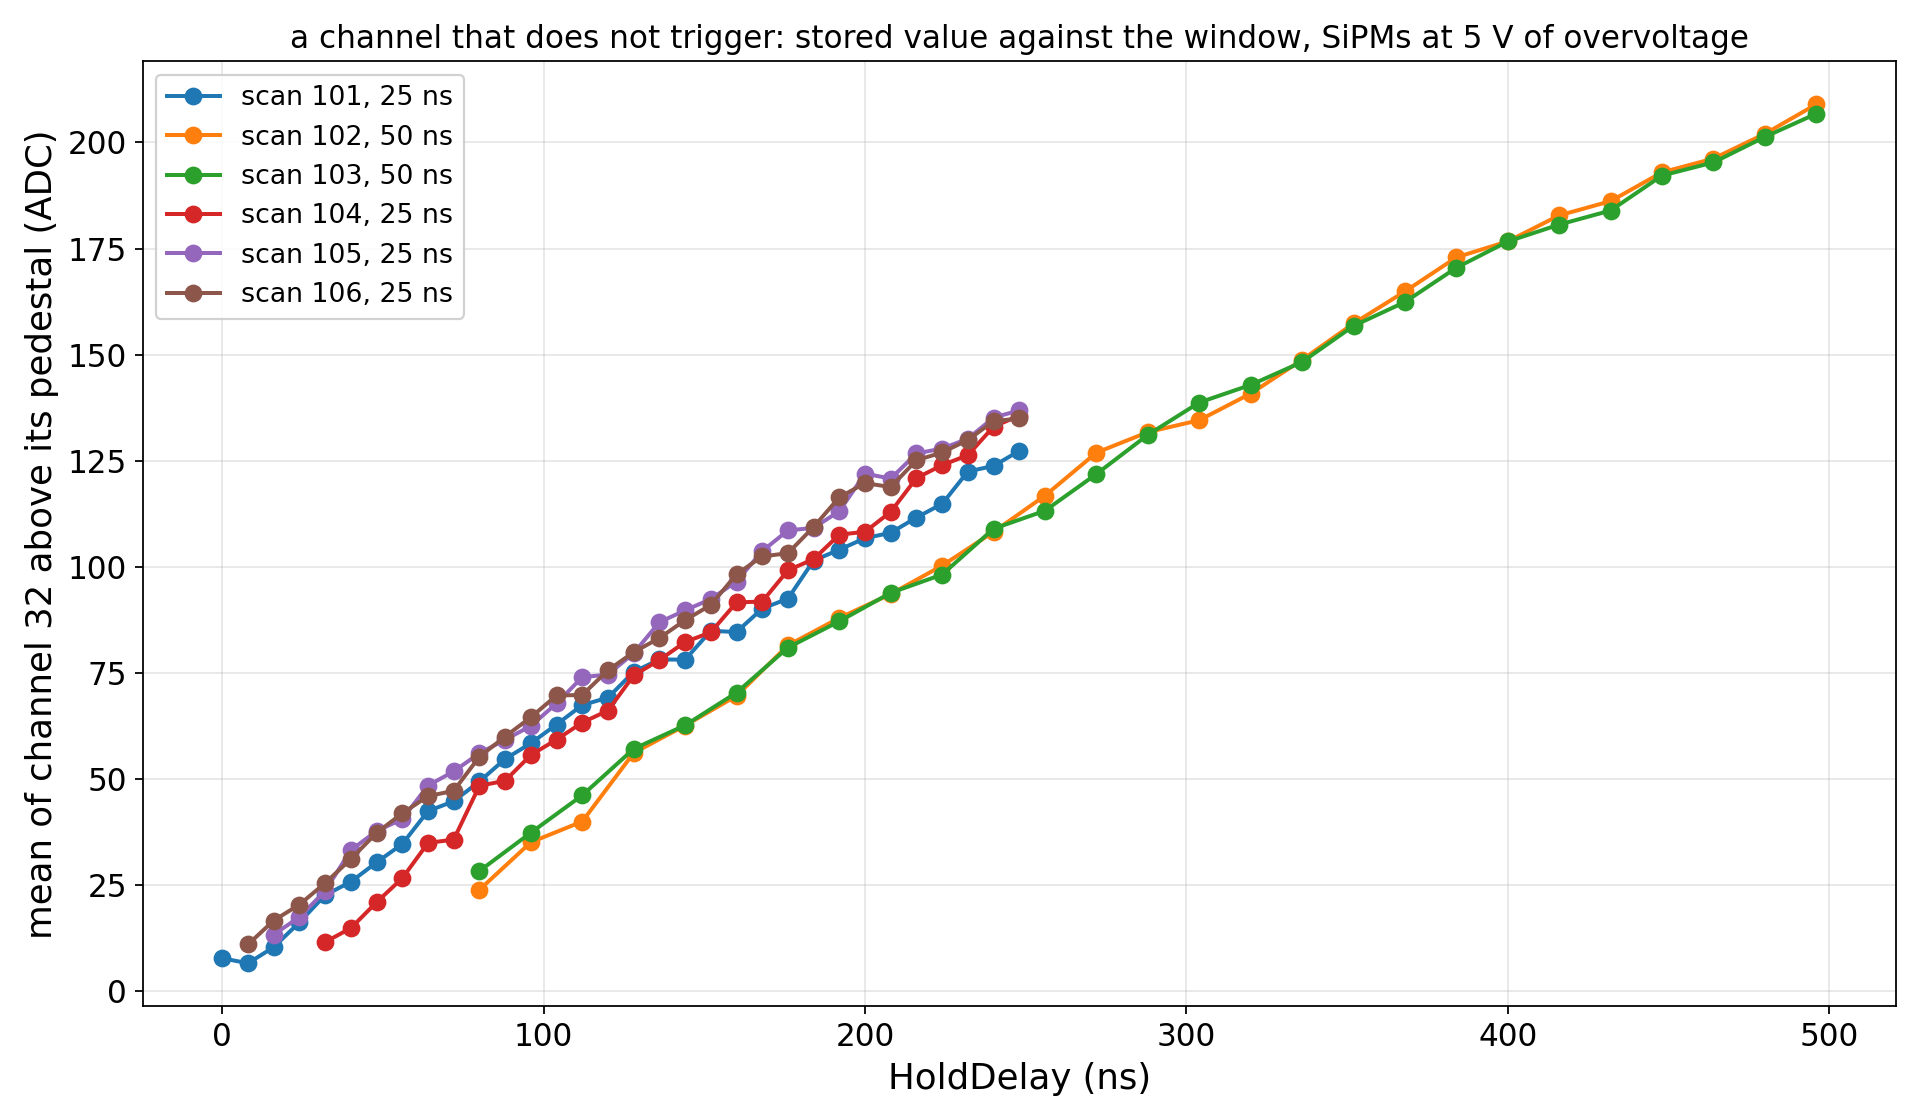
\includegraphics[width=\textwidth]{hold_scan_window.png}
\column{0.4\textwidth}
\begin{itemize}
\item The channels that do not trigger see the window at a random time with respect to their
  own dark pulses.
\item Their mean grows linearly with the window: 0.52 counts per ns at 25~ns, 0.42 at 50~ns.
\item At the gain above, 3.0 and 2.2 photoelectrons per microsecond.
\end{itemize}
\end{columns}
\end{frame}

\begin{frame}{Menu 2: values}
\begin{enumerate}
\item Threshold: edge of the noise at 179--182 DAC units at 5~V and 25~ns; one photoelectron
  is 20 units; the threshold of 185 is below one photoelectron.
\item Minimum hold delay: 40~ns at 25~ns of shaping, 160~ns at 50~ns.
\item Single-photoelectron gain at 5~V, high gain, preamplifier gain 55: 150--182 counts per
  photoelectron at 25~ns in the four channels scanned, 185--192 at 50~ns.
\item In a window at a random time, a channel at 5~V accumulates 3.0 photoelectrons per
  microsecond at 25~ns and 2.2 at 50~ns.
\end{enumerate}
\end{frame}

\end{document}
